\chapter{Model Validation} 

A very important task in the development of this software is to make sure that the results obtained by simulation agree reasonably well with real world examples.
This section shows the validation efforts made so far.
It is still very sparse, so if you have used this program for a real world application, let me know about your results and they will be added here.
\subsubsection{Statics of a straight steel bow}

In this experiment the draw curve and limb shapes of a small steel bow with a constant cross section have been measured and compared to version 2014.4 of Bow Simulation Tool (now VirtualBow).
The bow is shown in figure~\ref{fig:validation:setup} and has been made from an old saw blade.
Steel is a good material for this kind of test because of its homogenous mechanical properties.
The elastic modulus was assumed to be $E = 210\ \rm{GPa}$ which is a good estimate for most types of steel.

\begin{figure}[H]
\centering
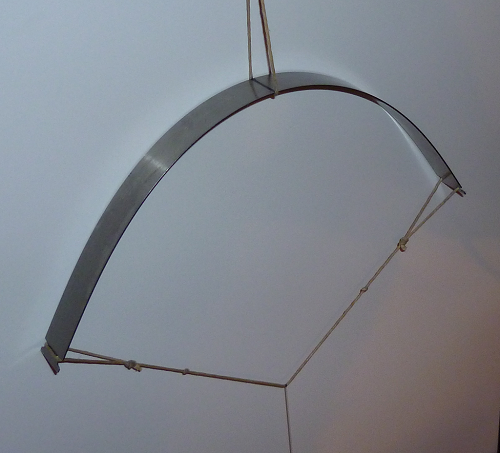
\includegraphics[width=0.5\textwidth]{figures/validation/setup.png}
\caption{Steel bow. Cross section:~16.85~$\times$~0.75mm. Length:~269mm. Brace heighth:~49.8mm}
\label{fig:validation:setup}
\end{figure}

The experiment was carried out by hanging a plastic bag at the string center.
The draw force was then gradually applied by counting steel balls with a known mass into the bag.
After every load step the draw length was measured and a photo of the bow was taken.

Figure~\ref{fig:validation:draw_curve} shows a comparison between the measured and the simulated draw curve and figure~\ref{fig:validation:limb_shapes} compares the pictures of the limb against the simulated limb shapes.

\begin{figure}[H]
\centering
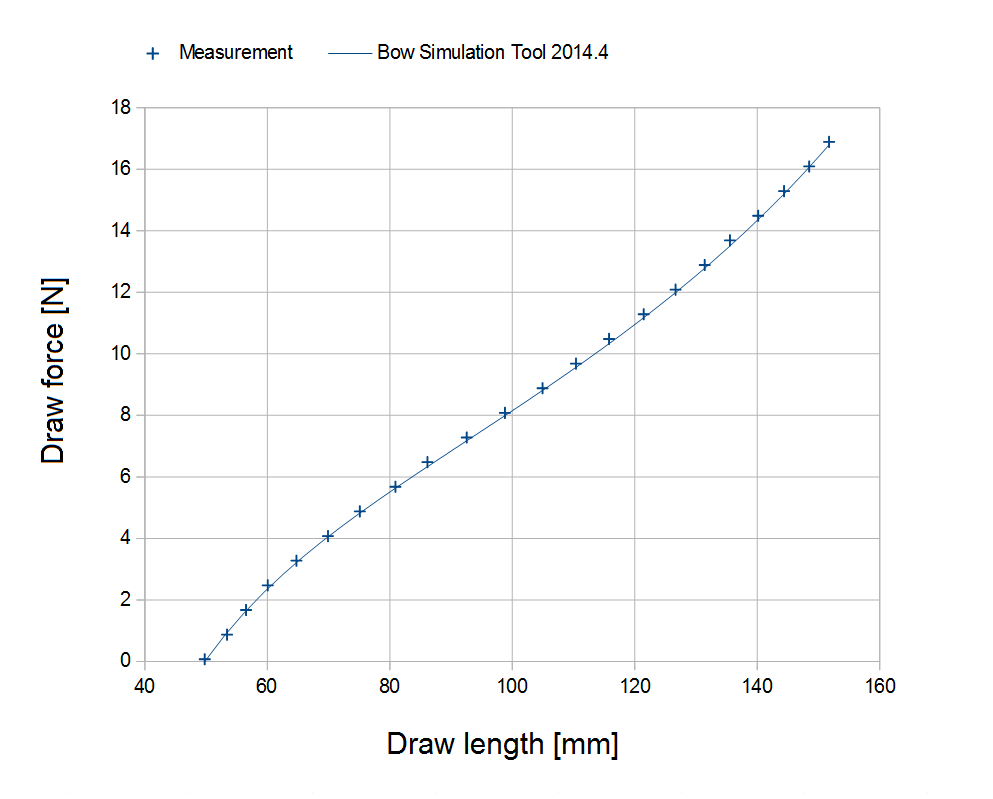
\includegraphics[width=0.85\textwidth]{figures/validation/draw_curve.png}
\caption{Experimental and simulated draw curves}
\label{fig:validation:draw_curve}
\end{figure}

\begin{figure}[H]
\centering
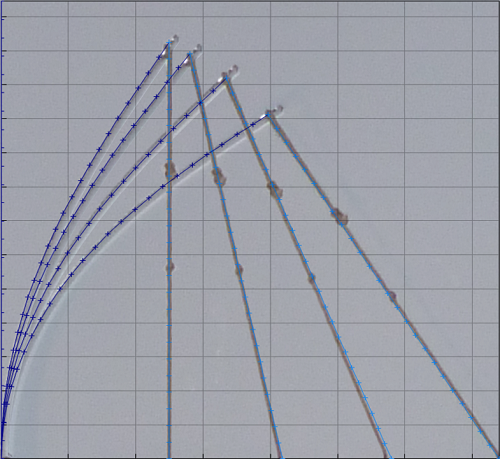
\includegraphics[width=0.65\textwidth]{figures/validation/states_blended.png}
\caption{Experimental and simulated limb shapes}
\label{fig:validation:limb_shapes}
\end{figure}

The agreement between experiment and simulation is surprisingly good here.
It really shows the potential of such kinds of simulations, provided that the material properties are well known and a the bow can be built exactly as simulated, with low tolerances.

But this is still a very simple example.
The next step would be to repeat this experiment with bows that have varying cross sections and non-straight profiles.
Another open question are the dynamic simulation results.
It's unclear if they can match experiments as good as the static results do, because there are much more uncertainties involved.